Carpenter~\cite{pan2003carpenter} è uno dei principali framework per
la ricerca di itemset su dataset ad alta dimensionalità.

Scopo dell'algoritmo è la ricerca di itemset colossali chiusi su dati ad alta dimensionalità.
Questo algoritmo individua insiemi di feature frequenti generando una versione trasposta del dataset originale, chiamata \textit{TT}, e un albero, chiamato \textit{row enumeration tree} avente nei nodi tutti i possibili set di transazioni;
successivamente questo viene esplorato utilizzando una ricerca \textit{depth-first}.

Il punto di partenza di Carpenter consiste in un insieme di transazioni \(D\) che contiene \(F\) attributi possibili.
Su questo sono definite due funzioni: si definisce funzione di calcolo del supporto di un set di attributi \(\mathcal{R}\) la funzione che dato un insieme di attributi \(F'\) calcola il numero totale di righe che li contiene.
Si noti che \(\mathcal{R}\) è analogo alla funzione \(s\), che dato un itemset ne calcola il supporto, presentata nella \cref{sec:fim}.
Analogamente si definisce funzione di calcolo del supporto comune ad un insieme di righe \(\mathcal{F}\) la funzione che dato un set di righe \(R'\) calcola il massimo insieme di item comune tra queste.
Preso come riferimento il dataset in \cref{fig:chap-3:carpenter-tt}, dato \(F' = (a,e,h)\), \(\mathcal{R}(F') = {2,3,4}\).
Dato invece il set di righe \(R' = (2,3)\), il set di feature corrispondenti risulta uguale a \(\mathcal{F}(R') = {a,e,h}\).

Una volta definite queste due funzioni di supporto, vine definita una tabella trasposta \textit{TT} sulla base del dataset originale.
In questa tabella le righe rappresentano le possibili feature e sono denominate tuple, mentre nelle colonne sono presenti gli id transazioni originali del dataset.
Un esempio di questa tabella è disponibile nella~\cref{fig:chap-3:carpenter-tt}.

\begin{figure}
  \centering
  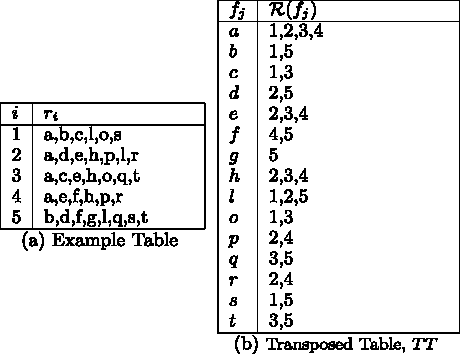
\includegraphics[width=0.5\textwidth]{res/fig/sec-3/DatasetAndTT.pdf}
  \caption{Esempio di tabella originale (a) e tabella trasposta (b), Fonte:~\cite{pan2003carpenter}}%
  \label{fig:chap-3:carpenter-tt}
\end{figure}

A differenza dei classici algoritmi di itemset mining, che esplorano lo spazio di ricerca tramite un enumerazione degli attributi, Carpenter esegue la ricerca sulla base di un enumerazione delle righe.
Questo approccio, nel caso di dataset ad alta dimensionalità, riduce lo spazio di ricerca.
Preso come esempio il dataset in~\cref{fig:chap-3:carpenter-tt} (figura a), nella \cref{subsec:apriori} si era dimostrato come una ricerca con l'algoritmo Apriori potesse potenzialmente generare \(32768\) candidati da valutare.
Una ricerca basata su righe implica considerare tutte le possibili combinazioni di righe.
Avendo il dataset in questione \(5\) righe, il numero di itemset da valutare sarà nel caso peggiore di \(32\), di tre ordini di grandezza inferiore rispetto a quello ottenuto con Apriori.

La~\cref{fig:chap-3:carpenter-ret} mostra il row enumeration tree, contenente il set completo di tutte le possibili combinazioni tra righe.
Questo albero è costruito enumerando tutte le possibili combinazioni di righe e disponendole in modo tale che ogni elemento di livello uno contenga nel suo sotto-albero tutte le possibili combinazioni tra se stesso e tutti gli elementi aventi ID maggiore del proprio.

\begin{figure}
  \centering
  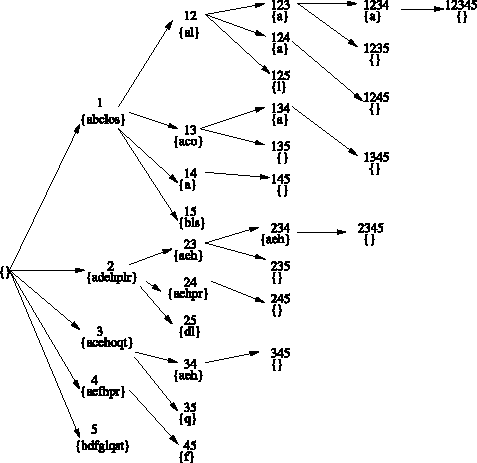
\includegraphics[width=.5\textwidth]{res/fig/sec-3/RowEnumerationTree.pdf}
  \caption{Esempio di Row Enumeration Tree, Fonte:~\cite{pan2003carpenter}}%
  \label{fig:chap-3:carpenter-ret}
\end{figure}

Per trovare i pattern chiusi e frequenti, Carpenter esegue una ricerca depth first, ovvero in cui viene stabilito un ordine lessicografico tra le transazioni e partendo da quelle avente indice più basso si esplora completamente il ramo delle possibilità collegate alla singola transazione.
Ogni elemento viene esplorato considerando solo gli elementi successivi, mai i precedenti.
In questo modo ogni possibile combinazione di righe è considerata una e una sola volta.
Ad ogni combinazione di righe è associato uno e un solo itemset chiuso, l'insieme di tutti gli itemset chiusi viene coperto considerando tutte le possibili combinazioni di righe.

Per eseguire la ricerca di itemset, poste queste condizioni, sarebbe sufficiente generare tutti le possibili combinazioni di righe, generare il loro set di attributi comuni applicando \(\mathcal{F}\) e valutare la frequenza di questo itemset.
Ciò però non sarebbe efficiente in quanto non verrebbe applicata la proprietà monotona del supporto.
Occorre quindi definire una strategia di pruning per ridurre lo spazio di ricerca.

Sia \(X\) un sottoinsieme di righe.
Data la tabella trasposta \(TT\) si definisce tabella trasposta condizionata a \(X\), denominata \(TT|_{X}\) un subset di righe di \(TT\) tale che:

\begin{enumerate}
    \item Per ogni tupla \(x\) che contiene tutti gli elementi di \(X\), esiste una tupla corrispondente in \(TT|_{X}\).
    \item Ogni tupla di \(TT|_{X}\) contiene solo elementi tali che il loro identificatore di riga è maggiore di qualunque elemento presente in \(X\).
\end{enumerate}

La \cref{fig:chap-3:carpenter-ttt} è un esempio di tabella trasposta per le transazioni \((2,3)\) del dataset in \cref{fig:chap-3:carpenter-tt}

\begin{figure}
  \centering
  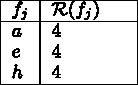
\includegraphics[width=.5\textwidth]{res/fig/sec-3/TT23.pdf}
  \caption{Tabella trasposta \(TT_{(2,3)}\) per l'insieme di transazioni \((2, 3)\), Fonte:~\cite{pan2003carpenter}}%
  \label{fig:chap-3:carpenter-ttt}
\end{figure}


Terminate le premesse, viene presentato il flusso dell'algoritmo di Carpenter (\cref{alg:carpenter}).

\begin{algorithm}[H]
\caption{Algoritmo di Carpenter}\label{alg:carpenter}
\begin{algorithmic}[1]
\Require \(F\): insieme degli attributi totali sul dataset, \(TT\): tabella trasposta, \(minsup\): soglia del supporto minimo
\Ensure \(FCP\): Pattern frequenti e chiusi

\State \(FCP \gets \varnothing\); \Comment{Inizializza l'output}
\State Dichiara R come l'insieme delle transazioni nel dataset originale ordinate per id;
\State$ MinePattern(TT|_{\varnothing}, R, FCP)$;
\State \Return \(FCP\)
\end{algorithmic}
\end{algorithm}

La logica di espansione e pruning di un itemset è contenuta all'interno del metodo \(MinePattern\) (\cref{alg:minepattern}).
In questi passi infatti viene valutata la creazione di un superset di un insieme di righe e la sua eventuale frequenza.
Durante il problema, sono definiti come \(I\) un itemset da valutare, \(X\) l'insieme delle righe che supportano \(I\) e \(R\) l'insieme delle righe da esplorare. 
Nel passo 1 dell'algoritmo viene calcolato il supporto di ogni riga \(r_i \in R\) all'interno della tabella trasposta \(TT|_X\).
A questo punto sono valutati in sequenza tre vincoli di pruning, il cui scopo è mantenere gli itemset chiusi non ancora esplorati:

\begin{enumerate}
    \item \textbf{Valutazione del superset dell'attuale set di transazioni} (passo 2).
    In questo passo viene ricercato il superset di \(X\) aggiungendo elementi di \(R\) tali che questi compaiano in almeno una riga di \(TT|_X\).
    Considerando tutti gli \(r_i,\ldots,r_n\) che soddisfano questa condizione, viene definito un superset di \(X\) \(EX = X \cup r_i \cup \ldots \cup r_n\).
    A questo punto se un superset di \(X\) non raggiunge la soglia minima di supporto, allora nessun itemset associato a una qualunque combinazione di queste righe potrà essere frequente.
    Preso come esempio il dataset in \cref{fig:chap-3:carpenter-tt} e posto \(minsup = 3\), si consideri \(X = \{3\}\) e \(R = \{4,5\}\).
    Da questo X viene generato un solo superset \(EX = \{3,4\}\), in quanto \(5\) non compare in nessuna delle transazioni di \(TT|_3\).
    Essendo \(|EX| < 3\), il processo legato all'esplorazione di questo ramo viene interrotta.
    È intuibile dalla \cref{fig:chap-3:carpenter-ret} che questo superset non potrà mai generare nessun itemset valido di \(3\) elementi.
    
    Formalmente si ricercano dentro \(R\) tutte le transazioni che compaiono in almeno una tupla di \(TT|_{X}\).
    Questo insieme viene definito come \(U\).
    Se la cardinalità di \(X \cup U\) risulta minore di \(minsup\), allora non potrà essere generato nessun itemset frequente nel superset, quindi l'esplorazione potrà essere interrotta.
    In caso contrario \(R' = U\). 
    Riferendosi all'esempio di prima \(U = {4}\), \(|X| + |U| = 2 < 3\), quindi è verificato quanto intuito sopra.
    
    \item \textbf{Eliminazione delle righe presenti in ogni tupla} (passo 3).
    Successivamente sono eliminate dall'insieme delle espansioni quelle righe che compaiono in ogni tupla della tabella trasposta \(TT|_X\).
    Questo potrebbe inizialmente sembrare un controsenso, eliminare una riga in cui \(I\) può essere espanso senza perdere elementi sembrerebbe uno sbaglio.
    Proprio per questo motivo in realtà queste righe vanno scartate.
    Scopo della creazione dei superset non è il conteggio del supporto di pattern già esistenti, quanto più l'individuare nuovi itemset non ancora valutati.
    Preso ad esempio \(X = (2,3), R = (4,5)\), \(\mathcal{F}(2,3) = \mathcal{F}(2,3,4)\) quindi la valutazione di \((2,3,4)\) non è necessaria, in quanto produrrebbe un itemset già visitato.
    
    In termini formali, le righe presenti in ogni tupla di \(TT|_X\) sono raccolte nell'insieme \(Y\), successivamente \(R' = R' - Y\).
    
    \item \textbf{Pruning degli itemset frequenti già esplorati} (passo 4).
    Ultimo passo di pruning, l'itemset che sta venendo considerato è già presente in \(FCP\), allora si può interrompere la ricerca su quel ramo.
    Intuitivamente, la natura depth-first dell'algoritmo implica che se un itemset è già presente in \(FCP\), questo sia già stato generato in un passaggio precedente dell'algoritmo.
    Questo passo di ricerca ha considerato transazioni con id inferiore a quello delle transazioni correnti, quindi sicuramente ha incluso anche quelle attualmente considerate nel calcolo del supporto.
    Ne segue che ogni possibile superset di queste righe è già stata valutata.
    Di conseguenza l'esplorazione del ramo termina.
    
    Si consideri \(X = (3, 4) \; R = (5)\) nel dataset in \cref{fig:chap-3:carpenter-tt}, \(\mathcal{F}(X) = (a,e,h)\).
    Nel momento in cui viene analizzato \(X\), \((a,e,h)\) risulta già presente in \(FCP\), in quanto generato da \(X' = (2,3), R' = (4, 5)\).
    Fissato questo, è possibile aggiungere che il superset \(EX = (3,4,5)\) risulta già valutata in \(EX' = (2,3,4,5)\).
    Questo perché se \(EX\) contenesse qualche itemset valido, questo sarebbe già individuato in \(EX'\), in quanto le righe in \(X'\) hanno id minore o uguale di quelle in X e individuano lo stesso pattern.
\end{enumerate}

Una volta che un candidato supera i tre vincoli di pruning, può essere valutato come frequente e espanso.
Nel passo 5 se l'unione tra \(X\) e \(Y\) risulta frequente, \(I\) viene aggiunto a \(FCP\), questo passaggio garantisce la validità del secondo vincolo.
Infine nel passo 6, per ogni riga in \(R'\) si esegue ricorsivamente \(MinePattern\) aggiungendo a \(X r_{i}\) e calcolando \(TT|_{X}|_{r_{i}}\)

\begin{algorithm}[H]
 \selectlanguage{italian}%
\caption{\(MinePattern(TT|_{X}, R', FCP)\)}\label{alg:minepattern}
\begin{algorithmic}[1]
\State Calcolo del supporto per ogni riga \(r_{i} \in R'\) su \(TT\). Inizializzazione di \(Y = \varnothing\); 
\State  Sia \(U \subset R'\) un set di righe che compare almeno in una tupla di \(TT_{X}\). Se \(|U| + |X| \leq minsup\) \Return altrimenti \(R' = U\). \Comment{Primo passo di pruning}
\State  Sia \(Y\) il set di righe tali che \(\forall r_{i} \in Y, r_{i} \in t_{j} \forall t_{j} \in TT|_{X}\), \(R = R - Y\) \Comment{Secondo passo di pruning}
\State  Se \(\mathcal{F}(X) \in FCP\), \Return \Comment{Terzo passo di pruning}
  \If{\(|X| + |Y| \geq minsup\)} \Comment{Se l'itemset è frequente rispetto alla soglia di supporto}
     \State \(FCP \gets \mathcal{F}(X) \cup FCP\) \Comment{La tupla viene aggiunta a FCP} 
  \EndIf
 \ForEach{\(r_{i} \in R'\)} \Comment{Per ogni elemento esplorabile}
        \State $R' = R' - {r_i}$ 
        \State $MinePattern(TT|_{X}|_{r_{i}}, R', FCP)$ \Comment{Passo ricorsivo dell'algoritmo}
    \EndFor
\end{algorithmic}
\end{algorithm}

Al termine dell'esecuzione dell'algoritmo sono riportati all'utente tutti gli itemset così individuati.
